\documentclass[10pt]{article}
\usepackage[verbose, a4paper, hmargin=2.5cm, vmargin=2.5cm]{geometry}

\usepackage{fontspec}
\usepackage{ctex}
\usepackage{paratype}

\usepackage{amsmath}
\usepackage{amssymb}
\usepackage{amsfonts}
\usepackage{esint}
\usepackage{stmaryrd}

\usepackage[mathbf=sym]{unicode-math}
\setmainfont{STIX Two Text}
\setmathfont{STIX Two Math}

\setsansfont{Arial}
\setmonofont{Courier New}

\usepackage{makecell}
\usepackage{wasysym}
\usepackage{pifont}
\usepackage[export]{adjustbox}
\usepackage{graphicx}
\usepackage{mdframed}
\usepackage{booktabs,array,multirow}
\usepackage{tabularx}
\usepackage{hyperref}
\hypersetup{colorlinks=true, linkcolor=blue, filecolor=magenta, urlcolor=cyan,}
\urlstyle{same}
\usepackage[most]{tcolorbox}
\usepackage{tikz}

% 定义考点分析框
\newtcolorbox{analysisbox}[1][]{
  colback=blue!5,
  colframe=blue!50!black,
  fonttitle=\bfseries,
  title=#1,
  boxrule=0.5pt,
  arc=2mm,
  left=5pt,
  right=5pt,
  top=5pt,
  bottom=5pt
}

% 定义教学提示框
\newtcolorbox{tipbox}[1][]{
  colback=orange!5,
  colframe=orange!60!black,
  fonttitle=\bfseries,
  title=#1,
  boxrule=0.5pt,
  arc=2mm,
  left=5pt,
  right=5pt,
  top=5pt,
  bottom=5pt
}

\definecolor{mygray}{RGB}{240,240,240}
\tcbset{
  colback=mygray,
  boxrule=0pt,
}
\graphicspath{ {./images/} }
\newcommand{\HRule}{\begin{center}\rule{0.9\linewidth}{0.2mm}\end{center}}
\newcommand{\customfootnote}[1]{
  \let\thefootnote\relax\footnotetext{#1}
}
\newcommand{\lt}{\mathrel{<}}
\newcommand{\gt}{\mathrel{>}}
\newcommand*\circled[1]{\tikz[baseline=(char.base)]{\node[shape=circle,draw,inner sep=1.5pt] (char) {\small #1};}}
\setcounter{MaxMatrixCols}{256}
\begin{document}
\begin{center}
\Large\textbf{2026届浦东新区高三下二模数学试卷}\\[0.5em]
\normalsize\textit{（教师版·带考点分析与教学评价）}
\end{center}

\section*{一、填空题}

1. 已知全集 \(U = \left( {0, + \infty }\right)\) ，集合 \(A = \lbrack 2, + \infty )\) ，则 \({\complement }_{U}A =\) \_\_\_\_.

\textbf{【答案】} \(\left( {0,2}\right)\)

\textbf{【解析】} \(U = \left( {0, + \infty }\right) ,A = \lbrack 2, + \infty ),{\complement }_{U}A = \left( {0,2}\right)\) .

\begin{analysisbox}[考点分析]
\textbf{知识点}：集合的补集运算\\
\textbf{难度}：\(\star\) 基础题\\
\textbf{评价}：考查补集的基本概念。注意全集是 \((0, +\infty)\) 而非 \(\mathbb{R}\)，区间端点的开闭容易出错。
\end{analysisbox}

2. 若复数 \(z\) 满足 \(\left( {1 + \mathrm{i}}\right) z = {2\mathrm{i}}\) ，则复数 \(z =\) \_\_\_\_.

\textbf{【答案】} \(1 + \mathrm{i}\)

\textbf{【解析】} \(\because \left( {1 + \mathrm{i}}\right) z = 2\mathrm{i},\therefore z = \frac{2\mathrm{i}}{1 + \mathrm{i}} = \frac{2\mathrm{i}\left( {1 - \mathrm{i}}\right) }{\left( {1 + \mathrm{i}}\right) \left( {1 - \mathrm{i}}\right) } = 1 + \mathrm{i}\) ,

\begin{analysisbox}[考点分析]
\textbf{知识点}：复数的四则运算\\
\textbf{难度}：\(\star\) 基础题\\
\textbf{评价}：复数除法需要通过分母实数化（乘以共轭复数）来求解。本题计算量较小，是基础送分题。
\end{analysisbox}

3. 已知 \(f\left( x\right)  = \left\{  \begin{array}{l} \frac{1}{{x}^{3}},x < 0 \\  x + 1,x \geq  0 \end{array}\right.\) ,若 \(f\left( a\right)  =  - 2\) ，则实数 \(a\) 的值为\_\_\_\_.

\textbf{【答案】}-8

\textbf{【解析】}若 \(a < 0\) ,则 \({a}^{\frac{1}{3}} =  - 2\) ,解得 \(a =  - 8\)

若 \(a \geq  0\) ,则 \(a + 1 =  - 2\) ,解得 \(a =  - 3\) ,不满足 \(a \geq  0\)

综上 \(a =  - 8\)

\begin{analysisbox}[考点分析]
\textbf{知识点}：分段函数\\
\textbf{难度}：\(\star\star\) 中档题\\
\textbf{评价}：分段函数求参数值，需要分类讨论。易错点：忘记检验解是否满足分段条件，或混淆 \(\frac{1}{x^3}\) 与 \(x^{\frac{1}{3}}\)。
\end{analysisbox}

\begin{tipbox}[教学提示]
分段函数问题的通用解题步骤：
\begin{enumerate}
\item 根据函数值判断自变量所在区间
\item 在各区间内分别求解
\item 检验解是否满足区间条件（舍根）
\item 综合各区间结果得出最终答案
\end{enumerate}
\end{tipbox}

4. 在 \(\bigtriangleup  {ABC}\) 中，若 \(a = 7\) ， \(b = 8\) ， \(\cos C = \frac{13}{14}\) ，则 \(c =\) \_\_\_\_.

\textbf{【答案】} 3

\textbf{【解析】}由余弦定理 \({c}^{2} = {a}^{2} + {b}^{2} - {2ab}\cos C\) 得: \({c}^{2} = {49} + {64} - {104} = 9\) ,

所以 \(c = 3\)

\begin{analysisbox}[考点分析]
\textbf{知识点}：余弦定理\\
\textbf{难度}：\(\star\) 基础题\\
\textbf{评价}：余弦定理的直接应用。注意计算准确性，\(2 \times 7 \times 8 \times \frac{13}{14} = 104\)。
\end{analysisbox}

5. 某校高中三年级 600 名学生参加了区质量检测,已知数学检测成绩 \(X\) 服从正态分布 \(N\left( {{100},{\sigma }^{2}}\right)\) (试卷满分为 150 分). 统计结果显示, 数学检测成绩介于 80 分到 120 分之间的人数为 450 名, 则此次检测中成绩不低于 120 分的学生人数约为总人数的\_\_\_\_(精确到 0.1\%).

\textbf{【答案】}12.5\%

\textbf{【解析】}由 \(X \sim  N\left( {{100},{\sigma }^{2}}\right)\) 可知,正态分布曲线对称轴为 \(X = {100}\) ,

可知 \(P\left( {{80} < x < {120}}\right)  = \frac{450}{600} = \frac{3}{4}\) ,

所以 \(P\left( {{100} < X < {120}}\right)  = \frac{3}{8}\) ,可得 \(P\left( {X \geq  {120}}\right)  = \frac{1}{2} - \frac{3}{8} = \frac{1}{8}\) ,即成绩不低于 120 分的学生人数约为总人数的 12.5\%.

\begin{analysisbox}[考点分析]
\textbf{知识点}：正态分布\\
\textbf{难度}：\(\star\star\) 中档题\\
\textbf{评价}：正态分布的对称性应用。关键步骤：
\begin{itemize}
\item 利用对称性：\(P(80 < X < 120) = 2P(100 < X < 120)\)
\item 利用总概率为1：\(P(X \geq 120) = \frac{1}{2} - P(100 < X < 120)\)
\end{itemize}
\end{analysisbox}

\begin{tipbox}[教学提示]
正态分布问题要充分利用对称性。可画图辅助理解：以 \(\mu = 100\) 为对称轴，左右两侧各占 50\%。
\end{tipbox}

6. 已知直线 \(l\) 是曲线 \(y = \frac{3}{x + 1} + \ln x\) 在 \(x = 2\) 处的切线,则 \(l\) 的斜率为\_\_\_\_.

\textbf{【答案】} \(\frac{1}{6}\)

\textbf{【解析】}由 \(y = \frac{3}{x + 1} + \ln x\) ,所以 \({y}^{\prime } =  - \frac{3}{{\left( x + 1\right) }^{2}} + \frac{1}{x}\) ,

所以曲线在 \(x = 2\) 处的切线斜率为: \(k = {\left. {y}^{\prime }\right| }_{x = 2} =  - \frac{3}{{\left( 2 + 1\right) }^{2}} + \frac{1}{2} =  - \frac{1}{3} + \frac{1}{2} = \frac{1}{6}\) .

\begin{analysisbox}[考点分析]
\textbf{知识点}：导数的几何意义\\
\textbf{难度}：\(\star\) 基础题\\
\textbf{评价}：切线斜率即函数在该点的导数值。求导时注意 \((\frac{u}{v})' = \frac{u'v - uv'}{v^2}\) 和 \((\ln x)' = \frac{1}{x}\)。
\end{analysisbox}

7. 从 4 名男生 3 名女生中选取 3 人，依次进行面试，其中恰好有 1 名女生，则有\_\_\_\_种不同的面试方法.

\textbf{【答案】}108

\textbf{【解析】}第一步: 从 3 名女生中选取 1 名,有 \({\mathrm{C}}_{3}^{1} = 3\) 种选法,

第二步: 从 4 名男生中选取 2 名,有 \({\mathrm{C}}_{4}^{2} = 6\) 种选法,

第三步:选取的 3 人依次进行面试，则有 \({\mathrm{A}}_{3}^{3} = 6\) 种排法，

所以一共有 \({\mathrm{C}}_{3}^{1}{\mathrm{C}}_{4}^{2}{\mathrm{\;A}}_{3}^{3} = 3 \times  6 \times  6 = {108}\) 种不同的面试方法.

\begin{analysisbox}[考点分析]
\textbf{知识点}：排列组合\\
\textbf{难度}：\(\star\star\) 中档题\\
\textbf{评价}：分步计数原理的应用。本题包含"选"和"排"两个环节：先组合选人，再排列定顺序。学生容易漏掉排列步骤。
\end{analysisbox}

8. 一个家庭有两个孩子，生肖均为十二生肖之一(等可能). 已知其中一个孩子属马，则另一个孩子也属马的概率为\_\_\_\_.

\textbf{【答案】} \(\frac{1}{23}\)

\textbf{【解析】}两个孩子的生肖组合有 \({12} \times  {12} = {144}\) 种,

记事件 A ``其中一个孩子属马'', 事件 B ``两个孩子都属马'',

则 \(\mathrm{P}\left( A\right)  = 1 - \frac{{11} \times  {11}}{144} = \frac{23}{144},\mathrm{P}\left( {AB}\right)  = \frac{1 \times  1}{144} = \frac{1}{144}\) ,

所以 \(P\left( {B \mid  A}\right)  = \frac{P\left( {AB}\right) }{P\left( A\right) } = \frac{\frac{1}{144}}{\frac{23}{144}} = \frac{1}{23}\) .

\begin{analysisbox}[考点分析]
\textbf{知识点}：条件概率\\
\textbf{难度}：\(\star\star\) 中档题\\
\textbf{评价}：经典的条件概率问题。关键是用对立事件求 \(P(A)\)："至少一个属马" = 1 - "两个都不属马"。也可用直观理解：已知至少一个属马，样本空间缩小为 23 种（12+12-1），其中有利事件 1 种。
\end{analysisbox}

\begin{tipbox}[教学提示]
本题是"boy or girl paradox"的变形。可对比讲解：
\begin{itemize}
\item "已知老大属马，老二属马的概率" = \(\frac{1}{12}\)
\item "已知至少一个属马，两个都属马的概率" = \(\frac{1}{23}\)
\end{itemize}
区别在于是否指定了特定孩子。
\end{tipbox}

9. 已知数列 \(\left\{  {a}_{n}\right\}\) 的通项公式是 \({a}_{n} = {2}^{n - 1} + 1,{S}_{n}\) 为数列 \(\left\{  {a}_{n}\right\}\) 的前 \(n\) 项和,则使得不等式 \({S}_{n} > {2026}\) 成立的最小正整数 \(n\) 的值为\_\_\_\_.

\textbf{【答案】}11

\textbf{【解析】}令 \({b}_{n} = {2}^{n - 1}\) ,则 \(\frac{{b}_{n + 1}}{{b}_{n}} = \frac{{2}^{n}}{{2}^{n - 1}} = 2\) ,

所以数列 \(\left\{  {b}_{n}\right\}\) 是以 \({b}_{1} = 1\) 为首项,2 为公比的等比数列,

设数列 \(\left\{  {b}_{n}\right\}\) 的前 \(n\) 项和为 \({T}_{n}\) ,则 \({T}_{n} = \frac{1 \times  \left( {1 - {2}^{n}}\right) }{1 - 2} = {2}^{n} - 1\) ,

所以 \({S}_{n} = {}_{1} + {}_{2} + \cdots  + {}_{n} = {}_{1} + 1 + {}_{2} + 1 + \cdots  + {}_{n} + 1 = 2{}^{n} - 1 + n\) ,

因为 \(y = {2}^{n} - 1 + n\) 单调递增,

又 \({S}_{10} = {1024} - 1 + {10} = {1033} < {2026},{S}_{11} = {2048} - 1 + {11} = {2058} > {2026}\) ,

所以使得不等式 \({S}_{n} > {2026}\) 成立的最小正整数 \(n\) 的值为 11 .

\begin{analysisbox}[考点分析]
\textbf{知识点}：等比数列求和、分组求和\\
\textbf{难度}：\(\star\star\) 中档题\\
\textbf{评价}：分组求和法的应用。将数列拆分为等比数列 \(\{2^{n-1}\}\) 和常数列 \(\{1\}\) 分别求和。最后通过估算确定 \(n\) 的值，体现"估算优于硬算"的数学思想。
\end{analysisbox}

10. 已知,圆 \(O\) 是圆心在原点的单位圆,弦 \({AB}\) 平行于 \(x\) 轴,并将圆分为两段弧. 将其中一段劣弧 \(\overset{\text{ ⏜ }}{AB}\) 沿弦 \({AB}\) 翻折后恰好经过圆心. 若直线 \(y = x + m\) 与翻折后得到的两段弧有四个不同的交点,则实数 \(m\) 的取值范围为\_\_\_\_.

\begin{center}
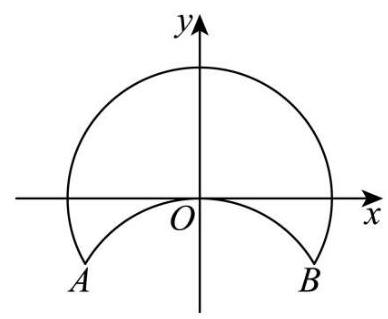
\includegraphics[max width=0.3\textwidth]{images/bo_d7ffgrqlb0pc73deo6k0_2_1121_1123_388_319_0.jpg}
\end{center}

\textbf{【答案】} \(\left( {\frac{\sqrt{3} - 1}{2},\sqrt{2} - 1}\right)\)

\textbf{【解析】}根据题意可知优弧 \({AB}\) 所在的圆方程为 \({x}^{2} + {y}^{2} = 1\) ,

劣弧 \({AB}\) 所在的圆方程为 \({x}^{2} + {\left( y + 1\right) }^{2} = 1\) ,

因为直线 \(y = x + m\) 与翻折后得到的两段弧有四个不同的交点,

所以直线 \(y = x + m\) 与优弧 \({AB}\) 和劣弧 \({AB}\) 各有两个不同的交点,

所以 \(\left\{  \begin{array}{l} \frac{\left| m\right| }{\sqrt{2}} < 1 \\  \frac{\left| 1 + m\right| }{\sqrt{2}} < 1 \end{array}\right.\) ,解得 \(- \sqrt{2} < m < \sqrt{2} - 1\) ,

又直线 \(y = x + m\) 经过点 \(A\left( {-\frac{\sqrt{3}}{2}, - \frac{1}{2}}\right)\) 时, \(m =  - \frac{1}{2} - \left( {-\frac{\sqrt{3}}{2}}\right)  = \frac{\sqrt{3} - 1}{2}\) ,

所以要使直线 \(y = x + m\) 与翻折后得到的两段弧有四个不同的交点,

\(m\) 的取值范围为 \(\left( {\frac{\sqrt{3} - 1}{2},\sqrt{2} - 1}\right)\)

\begin{analysisbox}[考点分析]
\textbf{知识点}：圆的方程、直线与圆的位置关系\\
\textbf{难度}：\(\star\star\star\) 难题\\
\textbf{评价}：解析几何综合题，考查空间想象能力。
\begin{itemize}
\item 关键突破：理解"劣弧翻折后过圆心"的几何意义，转化为圆的方程
\item 劣弧翻折后所在圆的圆心为 \((0, -1)\)，半径仍为 1
\item 四个交点的条件：直线与两个圆各有两个交点
\item 临界情况：直线过交点 \(A\)（或 \(B\)）时，交点个数变化
\end{itemize}
\end{analysisbox}

\begin{tipbox}[教学提示]
本题需要画图辅助理解。建议：
\begin{enumerate}
\item 先画单位圆，标出翻折后的劣弧所在位置
\item 确定劣弧端点 \(A, B\) 的坐标：\((-\frac{\sqrt{3}}{2}, -\frac{1}{2})\) 和 \((\frac{\sqrt{3}}{2}, -\frac{1}{2})\)
\item 分析直线 \(y = x + m\) 平移时交点个数的变化
\item 特别注意：直线不能过 \(A, B\) 点，否则交点会重合
\end{enumerate}
\end{tipbox}

11. 某光影科技实验室为长方体空间, 底面是边长为 4 米的正方形, 高为 3 米. 为营造动态光影效果, 在底面一个顶点处安装射灯 \(A\) ,在与该顶点相对的侧棱上、距底面 1 米处安装射灯 \(I\) ,两盖射灯的光束方向由智能系统自动控制，始终使两束光线相互垂直，且它们的交汇点 \(G\) 始终落在实验室天花板上，则交汇点 \(G\) 形成的轨迹长度为\_\_\_\_米.

\begin{center}
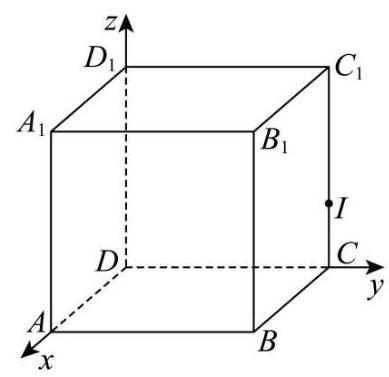
\includegraphics[max width=0.3\textwidth]{images/bo_d7ffgrqlb0pc73deo6k0_3_1106_539_389_377_0.jpg}
\end{center}

\textbf{【答案】} \(2\sqrt{2}\pi\)

\textbf{【解析】}如图建立空间直角坐标系:

则 \(A\left( {4,0,0}\right) , I\left( {0,4,1}\right)\) ,设交点 \(G\left( {x, y,3}\right)\) ,

所以 \(\overrightarrow{AG} = \left( {x - 4, y,3}\right) ,\overrightarrow{IG} = \left( {x, y - 4,2}\right)\) ,

因为 \({AG} \bot  {IG}\) ,所以 \(\overrightarrow{AG} \cdot  \overrightarrow{IG} = \left( {x - 4}\right) x + \left( {y - 4}\right) y + 3 \times  2 = 0\) ,

整理得 \({\left( x - 2\right) }^{2} + {\left( y - 2\right) }^{2} = 2\) ,

所以交点 \(G\) 在天花板上的轨迹是以 \(\left( {2,2,3}\right)\) 为圆心,半径为 \(\sqrt{2}\) 的圆,

所以交汇点 \(G\) 形成的轨迹长度为 \(2\sqrt{2}\pi\) .

\begin{analysisbox}[考点分析]
\textbf{知识点}：空间向量、立体几何\\
\textbf{难度}：\(\star\star\star\) 难题\\
\textbf{评价}：空间几何与解析几何的综合题。
\begin{itemize}
\item 关键：建立合适的空间直角坐标系
\item 利用向量垂直条件 \(\overrightarrow{AG} \cdot \overrightarrow{IG} = 0\) 建立方程
\item 化简得到圆的方程，求圆周长
\item 考查空间想象能力和计算能力
\end{itemize}
\end{analysisbox}

\begin{tipbox}[教学提示]
本题是立体几何与解析几何的跨模块综合题。
\begin{enumerate}
\item 强调坐标系的建立原则：尽量利用已知垂直关系
\item 点 \(G\) 在天花板上意味着 \(z = 3\)，这是重要约束条件
\item 向量垂直的坐标表示要熟练
\item 轨迹问题的一般思路：设点→列方程→化简→识别曲线类型
\end{enumerate}
\end{tipbox}

12. 已知集合 \(M\) 的元素均为正整数，定义集合 \(M\) 的"变项和"为:将 \(M\) 中每个元素 \(m\) 都乘以 \({\left( -1\right) }^{m}\) 后再求和. 若集合 \(A = \{ n \mid  1 \leq  n \leq  {2026},n \in  \mathbf{N}\}\) ，则集合 \(A\) 的所有非空子集的"变项和"的总和为\_\_\_\_.

\textbf{【答案】} \({1013} \times  {2}^{2025}\)

\textbf{【解析】}: \(A = \left\{  {n \mid  1 \leq  n \leq  {2026}, n \in  \mathbf{N}}\right\}   = \{ 1,2,\cdots ,{2026}\}\) ,

\(\therefore A\) 中所有非空子集含有 1 的有 2026 类:

单元素集合只有 \(\{ 1\}\) 含有 1,即 1 出现了 \({\mathrm{C}}_{2025}^{0}\) 次;

双元素集合含有 1 的有 \(\{ 1,2\} ,\{ 1,3\} ,\ldots \{ 1,{2026}\}\) ,即 1 出现了 \({\mathrm{C}}_{2025}^{1}\) 次;

三元素集合中含有 1 的有 \(\{ 1,2,3\} ,\{ 1,2,4\} ,\cdots ,\{ 1,{2025},{2026}\}\) ,即 1 出现了 \({\mathrm{C}}_{2025}^{2}\) 次,

......

有 2026 个元素的集合中含有 1 的有 \(\{ 1,2,\cdots ,{2026}\}\) ，1 出现了 \({\mathrm{C}}_{2025}^{2025}\) 次；

\(\therefore 1\) 共出现 \({\mathrm{C}}_{2025}^{0} + {\mathrm{C}}_{2025}^{1} + \ldots  + {\mathrm{C}}_{2025}^{2025} = {2}^{2025}\) ,

同理 \(2,3,4,\cdots {2026}\) 都出现 \({2}^{2025}\) 次,

\(\therefore M\) 的所有非空子集中,这些和的总和是

\[
{2}^{2025} \times  \left\lbrack  {1 \times  {\left( -1\right) }^{1} + 2 \times  {\left( -1\right) }^{2} + \cdots  + {2026} \times  {\left( -1\right) }^{2026}}\right\rbrack
\]

\(= {2}^{2025} \cdot  \left\{  {\left\lbrack  {1 \times  {\left( -1\right) }^{1} + 2 \times  {\left( -1\right) }^{2}}\right\rbrack   + \left\lbrack  {3 \times  {\left( -1\right) }^{3} + 4 \times  {\left( -1\right) }^{4}}\right\rbrack   + \cdots  + \left\lbrack  {{2025} \times  {\left( -1\right) }^{2025} + {2026} \times  {\left( -1\right) }^{2026}}\right\rbrack  }\right\}\)

\[
= {2}^{2025} \times  \left( {1 + 1 + \cdots  + 1}\right)  = {2}^{2025} \times  {1013}.
\]

\begin{analysisbox}[考点分析]
\textbf{知识点}：集合、二项式定理\\
\textbf{难度}：\(\star\star\star\star\) 压轴题\\
\textbf{评价}：本题是填空题的压轴题，综合性极强。
\begin{itemize}
\item 核心思想：每个元素在所有非空子集中出现的次数相同
\item 利用二项式定理：\(\sum_{k=0}^{n} C_n^k = 2^n\)
\item "变项和"的定义创新，需要准确理解
\item 最后求和时利用分组配对，每对和为 1
\end{itemize}
\end{analysisbox}

\begin{tipbox}[教学提示]
本题是典型的"新定义"压轴题。
\begin{enumerate}
\item 首先让学生准确理解"变项和"的定义
\item 关键突破口：思考每个元素在多少个子集中出现
\item 推广思考：若集合有 \(n\) 个元素，每个元素出现 \(2^{n-1}\) 次
\item 本题是求所有非空子集的"变项和"之和，不是求某个特定子集
\item 最后一问：\((-2k+1)(-1) + (2k)(1) = 1\)，共 1013 组
\end{enumerate}
\end{tipbox}

\section*{二、单选题}

13. 某校学生会体育部长依据本校高三男生的身高(单位:cm)与体重(单位:kg)的抽样数据，运用电子办公软件求出了"体重"(y)关于"身高"(x)的回归方程，则该回归方程()

身高体重

174 55

176 58

176 62

181 74

182 88

179 68

169 54

168 52

171 56

180 86

\begin{center}
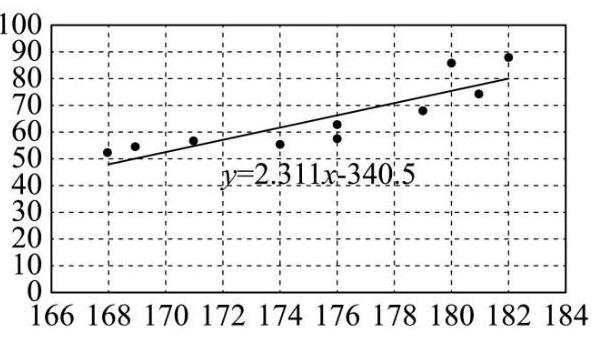
\includegraphics[max width=0.5\textwidth]{images/bo_d7ffgrqlb0pc73deo6k0_4_350_751_593_337_0.jpg}
\end{center}

A. 表示 \(x\) 与 \(y\) 之间的函数关系 B. 表示 \(x\) 与 \(y\) 之间的不确定关系

C. 反映 \(x\) 与 \(y\) 之间的真实关系 D. 反映 \(x\) 与 \(y\) 之间的真实关系的一种最佳拟合

\textbf{【答案】}D

\textbf{【解析】}根据线性回归方程的概念可知,回归方程反映 \(x\) 与 \(y\) 之间的真实关系的一种最佳拟合.

\begin{analysisbox}[考点分析]
\textbf{知识点}：线性回归\\
\textbf{难度}：\(\star\) 基础题\\
\textbf{评价}：考查回归分析的基本概念。回归方程是对相关关系的最佳拟合，不是严格的函数关系。
\end{analysisbox}

14. 已知实数 \(a,b,c\) 满足 \(a > b > 1 > c\) ,则下列结论一定正确的是( )

A. \({ac} > {bc}\) B. \({b}^{c} < 1\)

C. \({\log }_{a}b + {\log }_{b}a > 2\) D. \(a + c > b\)

\textbf{【答案】}C

\textbf{【解析】}对于选项 \(\mathrm{A}\) ,可知 \(1 > c\) ,无法判断正负,所以选项 \(\mathrm{A}\) 错误;

对于选项 \(\mathrm{B}\) ,可知 \(0 < c < 1 < b\) 时,所以 \({b}^{c} > 1\) ,所以选项 \(\mathrm{B}\) 错误;

对于选项 \(\mathrm{C}\) ,因为 \(a > b > 1\) ,所以 \(\ln a > \ln b > 0\) ,

可知 \({\log }_{a}b + {\log }_{b}a = \frac{\ln b}{\ln a} + \frac{\ln a}{\ln b} \geq  2\sqrt{\frac{\ln b}{\ln a}\frac{\ln a}{\ln b}} = 2\) ,当且仅当 \(\frac{\ln b}{\ln a} = \frac{\ln a}{\ln b}\) ,即 \(a = b\) 时取等号,所以等号取不到, 所以 \({\log }_{a}b + {\log }_{b}a > 2\) ,选项 \(\mathrm{C}\) 正确;

对于选项 \(\mathrm{D}\) ,当 \(c < 0\) 时,无法判断不等式是否成立,所以选项 \(\mathrm{D}\) 错误;

\begin{analysisbox}[考点分析]
\textbf{知识点}：不等式、对数函数\\
\textbf{难度}：\(\star\star\) 中档题\\
\textbf{评价}：综合考查不等式性质和对数运算。
\begin{itemize}
\item 选项C是关键：利用换底公式和基本不等式
\item 注意等号条件 \(a=b\) 与题设 \(a>b\) 矛盾，所以严格大于2
\item 其他选项可通过举反例排除
\end{itemize}
\end{analysisbox}

\begin{tipbox}[教学提示]
此类选择题建议采用"排除法+直接证明"。
\begin{itemize}
\item 先分析哪个选项最有可能正确（通常是不等式证明）
\item 对于错误的选项，快速举反例：如A取 \(c=-1\)，B取 \(c=0.5\)，D取 \(c=-10\)
\item 强调基本不等式取等条件的检验
\end{itemize}
\end{tipbox}

15. 已知 \(\overrightarrow{{e}_{1}},\overrightarrow{{e}_{2}}\) 与 \(\overrightarrow{{e}_{3}}\) 是不共面的向量,则以下向量组中,一定不共面的是 ( )

A. \(\overrightarrow{{e}_{1}} + \overrightarrow{{e}_{2}}\text{ 、 }\overrightarrow{{e}_{3}}\text{ 、 }\overrightarrow{{e}_{1}} + \overrightarrow{{e}_{2}} + \overrightarrow{{e}_{3}}\)

B. \(\overrightarrow{{e}_{1}}\text{ 、 }\overrightarrow{{e}_{2}} + \overrightarrow{{e}_{3}}\text{ 、 }3\overrightarrow{{e}_{1}} + 4\overrightarrow{{e}_{2}} + 3\overrightarrow{{e}_{3}}\)

C. \(\overrightarrow{{e}_{1}}\text{ 、 }2\overrightarrow{{e}_{2}} - \overrightarrow{{e}_{3}}\text{ 、 }\overrightarrow{{e}_{1}} - 2\overrightarrow{{e}_{2}} + \overrightarrow{{e}_{3}}\)

D. \(\overrightarrow{{e}_{1}} + \overrightarrow{{e}_{2}}\text{ 、 }\overrightarrow{{e}_{2}} + \overrightarrow{{e}_{3}}\text{ 、 }\overrightarrow{{e}_{1}} + k\overrightarrow{{e}_{3}}\) (其中 \(k\) 为实数)

\textbf{【答案】}B

\textbf{【解析】}对于 \(\mathrm{A}\) ,设 \(\overrightarrow{{e}_{1}} + \overrightarrow{{e}_{2}} = x\overrightarrow{{e}_{3}} + y\left( {\overrightarrow{{e}_{1}} + \overrightarrow{{e}_{2}} + \overrightarrow{{e}_{3}}}\right)\) ,
由 \(\overrightarrow{{e}_{1}},\overrightarrow{{e}_{2}}\) 与 \(\overrightarrow{{e}_{3}}\) 是不共面的向量,方程组有解,所以共面,故 A 错误;

对于 \(\mathrm{B}\) ,设 \(\overrightarrow{{e}_{1}} = x\left( {\overrightarrow{{e}_{2}} + \overrightarrow{{e}_{3}}}\right)  + y\left( {3\overrightarrow{{e}_{1}} + 4\overrightarrow{{e}_{2}} + 3\overrightarrow{{e}_{3}}}\right)\) ,
由不共面向量条件得方程组 \(\left\{  \begin{array}{l} {3y} = 1 \\  x + {4y} = 0 \\  x + {3y} = 0 \end{array}\right.\) ,方程组无解, 所以不共面,故 B 正确;

对于 \(\mathrm{C}\) ,类似分析可得方程组有解 \(\left\{  \begin{array}{l} y = 1 \\  x = 1 \end{array}\right.\) ,所以共面,故 C 错误;

对于 \(\mathrm{D}\) ,当 \(k =  - 1\) 时方程组有解,此时向量共面,故 D 错误.

\begin{analysisbox}[考点分析]
\textbf{知识点}：空间向量、共面向量\\
\textbf{难度}：\(\star\star\star\) 难题\\
\textbf{评价}：空间向量共面性的判定。
\begin{itemize}
\item 核心方法：设 \(\vec{a} = x\vec{b} + y\vec{c}\)，若方程组有解则共面，无解则不共面
\item 注意：三个向量共面的充要条件是其中一个可由另外两个线性表示
\item 选项D含有参数 \(k\)，需要对 \(k\) 进行讨论
\end{itemize}
\end{analysisbox}

\begin{tipbox}[教学提示]
向量共面问题的解题策略：
\begin{enumerate}
\item 判断依据：若存在不全为零的实数 \(\lambda, \mu, \nu\) 使 \(\lambda\vec{a} + \mu\vec{b} + \nu\vec{c} = \vec{0}\)，则三向量共面
\item 实用方法：尝试将其中一个向量表示为另外两个的线性组合
\item 空间基底 \(\{\vec{e_1}, \vec{e_2}, \vec{e_3}\}\) 不共面，这是判断的基础
\end{enumerate}
\end{tipbox}

16. 定义在 \(\mathbf{R}\) 上的非常值函数 \(y = f\left( x\right)\) ,若存在一个非零常数 \(T\) ,使得对任意 \(x \in  \mathbf{R}\) ,都有 \(f\left( {x + T}\right)  = T \cdot  f\left( x\right)\) 成立,那么称函数 \(y = f\left( x\right)\) 为 \(T\) 函数. 则下列说法正确的是( )

A. 存在函数 \(y = {kx} + b\left( {k \neq  0}\right)\) 为 \(T\) 函数

B. 若函数 \(y = f\left( x\right)\) 为 \(T\) 函数,且当 \(T > 1\) 时函数在 \(\lbrack 0,T)\) 上是严格增函数,则函数 \(y = f\left( x\right)\) 在 \(\lbrack 0, + \infty )\) 上是严格增函数

C. 若函数 \(y = f\left( x\right)\) 为 \(T\) 函数,且在 \(x = 0\) 处取得最小值,则 \(0 < T < 1\)

D. 若函数 \(y = f\left( x\right)\) 为 \(T\) 函数,且 \(\left| {f\left( x\right) }\right|  \leq  1\) 恒成立,则 \(y = f\left( x\right)\) 为周期函数

\textbf{【答案】}D

\textbf{【解析】}对 \(\mathrm{A}\) : 由 \(k(x+T) + b = T(kx + b)\) 整理得 \(kx + kT + b = kTx + Tb\) ,
则有 \(k = kT\) 且 \(kT + b = Tb\)，由 \(k \neq 0\) 得 \(T = 1\)，此时 \(k + b = b\) 则 \(k = 0\)，矛盾,故 A 错误;

对 B: 假设 \(T = 2\)，当 \(x \in \lbrack 0,2)\) 时 \(f(x) = x - 1\) ,
则 \(f(2) = 2f(0) = -2\)，不满足在 \(\lbrack 0, +\infty)\) 上严格递增,故 B 错误;

对 C: 假设 \(T = 2\)，当 \(x \in \lbrack 0,2)\) 时 \(f(x) = x\) ,则 \(f(x+2) = 2f(x)\) ,
可以验证 \(f(x)\) 在 \(x = 0\) 处取得最小值,但 \(T = 2\)，故 C 错误;

对 D: 由 \(f(x + nT) = T^n f(x)\) 和 \(|f(x)| \leq 1\) 恒成立,
若 \(|T| > 1\) 或 \(|T| < 1\)，当 \(n\) 足够大时不等式不成立,
故必有 \(|T| = 1\)，即 \(T = 1\) 或 \(T = -1\)，都是周期函数,故 D 正确.

\begin{analysisbox}[考点分析]
\textbf{知识点}：函数性质、周期函数\\
\textbf{难度}：\(\star\star\star\) 难题\\
\textbf{评价}：新定义函数性质题，是选择压轴题。
\begin{itemize}
\item 核心是理解 \(T\) 函数的定义：\(f(x+T) = T \cdot f(x)\)
\item 注意与周期函数的区别：周期函数是 \(f(x+T) = f(x)\)
\item 选项D的证明需要用到有界性条件和反证法
\item 其他选项通过构造反例排除
\end{itemize}
\end{analysisbox}

\begin{tipbox}[教学提示]
新定义函数题的解题策略：
\begin{enumerate}
\item 首先准确理解定义，写出数学表达式
\item 尝试简单的函数类型（常数函数、一次函数、指数函数等）
\item 注意定义中的约束条件："非零常数 \(T\)"、"非常值函数"
\item 对于存在性问题，尝试构造；对于全称命题，尝试反例
\item 选项D是经典的有界性+递推型证明
\end{enumerate}
\end{tipbox}

\section*{三、解答题}

17. （14分）如图,在多面体 \({PQABCD}\) 中,平面 \({PAD} \bot\) 平面 \({ABCD},{AB}//{CD}//{PQ},{PD} \bot  {CD},\bigtriangleup {PAD}\) 是边长为 \(\sqrt{2}\) 的等边三角形, \({AB} = {PQ} = \frac{1}{2}{CD}\) .

\begin{center}
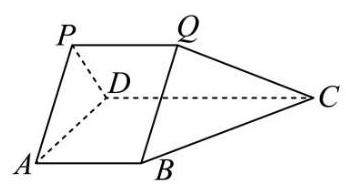
\includegraphics[max width=0.2\textwidth]{images/bo_d7ffgrqlb0pc73deo6k0_7_1158_1443_346_188_0.jpg}
\end{center}

(1)求证: \({AB}\bot\) 平面 \({PAD}\) ；

(2)若 \({PC}\) 与平面 \({ABCD}\) 所成的角为 \(\frac{\pi }{6}\) ，求多面体 \({PQABCD}\) 的体积.

\textbf{【答案】}(1)见解析; (2) \(\frac{2\sqrt{3}}{3}\)

\textbf{【解析】}(1) 证明: 取 \({AD}\) 的中点 \(O\) ,连接 \({PO}\) ,

因为 \(\bigtriangleup {PAD}\) 为等边三角形,且 \(O\) 为 \({AD}\) 中点,

所以 \({PO} \bot  {AD}\)

又平面 \({PAD} \bot\) 平面 \({ABCD}\) ,

平面 \({PAD} \cap\) 平面 \({ABCD} = {AD},{PO} \subset\) 平面 \({PAD}\) ,

所以 \({PO} \bot\) 平面 \({ABCD}\) .

又 \({AB} \subset\) 平面 \({ABCD}\) ,因而 \({PO} \bot  {AB}\)

因为 \({AB}//{CD},{PD} \bot  {CD}\) ,所以 \({PD} \bot  {AB}\)

由 \({PO} \subset\) 平面 \({PAD},{PD} \subset\) 平面 \({PAD},{PO} \cap  {PD} = P\) ,

所以 \({AB} \bot\) 平面 \({PAD}\) .

(2)连接 \({PC}\text{ 、 }{OC}\) ,由题(1)可知, \({PO} \bot\) 平面 \({ABCD}\) ,

所以 \({PC}\) 在平面 \({ABCD}\) 内的投影为 \({OC}\) ,

故 \(\angle {PCO}\) 是 \({PC}\) 与平面 \({ABCD}\) 所成的角,即 \(\angle {PCO} = \frac{\pi }{6}\)

\(\tan \angle {PCO} = \frac{PO}{CO} = \frac{\sqrt{3}}{3}\) ,由题得, \({PO} = \frac{\sqrt{6}}{2},{CO} = \frac{3\sqrt{2}}{2}\)

因为 \({AB} \bot\) 平面 \({PAD},{AB}//{CD}\) ,所以 \({CD} \bot\) 平面 \({PAD}\) ,所以 \({CD} \bot  {AD}\) .

因此, \({CD} = \sqrt{C{O}^{2} - O{D}^{2}} = 2,{PQ} = \frac{1}{2}{CD} = 1\)

取 \({CD}\) 的中点 \(M\) ,连接 \({BM}\text{ 、 }{QM}\) ,

则 \({V}_{PQABCD} = {V}_{{PAD} - {QBM}} + {V}_{Q - {MBC}}\)

\(= {AB} \cdot  {S}_{\bigtriangleup {PAD}} + \frac{1}{3}{CM} \cdot  {S}_{\bigtriangleup {QMB}} = \frac{\sqrt{3}}{2} + \frac{\sqrt{3}}{6} = \frac{2\sqrt{3}}{3}\)

所以多面体 \({PQABCD}\) 的体积是 \(\frac{2\sqrt{3}}{3}\) .

\begin{analysisbox}[考点分析]
\textbf{知识点}：立体几何、空间向量\\
\textbf{难度}：\(\star\star\star\) 难题\\
\textbf{评价}：解答题第一题，立体几何综合题。
\begin{itemize}
\item 第(1)问：线面垂直的证明，需要利用面面垂直的性质定理
\item 第(2)问：求体积，关键是确定几何体的形状和各边长
\item 利用线面角的定义找到 \(PC\) 与底面所成角
\item 体积计算采用分割法：将多面体分割为熟悉的几何体
\end{itemize}
\end{analysisbox}

\begin{tipbox}[教学提示]
立体几何解题要点：
\begin{enumerate}
\item 认真分析几何体的结构特征，明确各元素位置关系
\item 面面垂直性质定理：若两平面垂直，在一个平面内垂直于交线的直线垂直于另一平面
\item 线面角的找法：过斜线上一点作平面的垂线，连接垂足和斜足
\item 不规则多面体体积常用分割法或补形法
\end{enumerate}
\end{tipbox}

\newpage

18. （14分）已知 \(f\left( x\right)  = \sqrt{3}\sin x + 2\cos \left( {x + \varphi }\right) ,\varphi  \in  \left\lbrack  {0,\pi }\right\rbrack\) .

(1)若函数 \(y = f\left( x\right)\) 是定义在 \(\mathrm{R}\) 上的奇函数，求常数 \(\varphi\) 的值；

(2)若 \(\varphi  = \frac{\pi }{3}\) ，若关于 \(x\) 的不等式 \(f\left( x\right)  + \frac{x}{2} - a > 0\) 对任意 \(x \in  \left\lbrack  {0,\pi }\right\rbrack\) 恒成立，求实数 \(a\) 的取值范围.

\textbf{【答案】} \(\left( 1\right) \frac{\pi }{2};\left( 2\right) \left( {-\infty ,\frac{5\pi }{12} - \frac{\sqrt{3}}{2}}\right)\)

\textbf{【解析】}(1) 若函数 \(y = f\left( x\right)\) 是定义在 \(\mathbf{R}\) 上的奇函数,

则 \(f\left( {-x}\right)  =  - f\left( x\right)\) 对任意 \(x \in  \mathbf{R}\) 恒成立,

即 \(\sqrt{3}\sin x + 2\cos \left( {x + \varphi }\right)  =  - \sqrt{3}\sin \left( {-x}\right)  - 2\cos \left( {-x + \varphi }\right)\)

即 \(\cos \left( {x + \varphi }\right)  + \cos \left( {-x + \varphi }\right)  = 0\) 对 \(x \in  \mathbf{R}\) 恒成立.

即 \(2\cos x \cdot  \cos \varphi  = 0\) 对 \(x \in  \mathbf{R}\) 恒成立.

因此 \(\varphi  = {k\pi } + \frac{\pi }{2}\left( {k \in  \mathbf{Z}}\right)\) . 又 \(\varphi  \in  \left\lbrack  {0,\pi }\right\rbrack\) ,故 \(\varphi  = \frac{\pi }{2}\) .

因此,若函数 \(y = f\left( x\right)\) 是定义在 \(\mathbf{R}\) 上的奇函数,常数 \(\varphi\) 的值为 \(\frac{\pi }{2}\) ;

(2)若 \(\varphi  = \frac{\pi }{3}\) ，则 \(f\left( x\right)  = \cos x\) ，

由题意,即 \(a < \cos x + \frac{1}{2}x\) 对任意 \(x \in  \left\lbrack  {0,\pi }\right\rbrack\) 恒成立.

令 \(g\left( x\right)  = \cos x + \frac{1}{2}x\) ,即 \(a < g{\left( x\right) }_{\min }\) ,

由 \({g}^{\prime }\left( x\right)  = \frac{1}{2} - \sin x\) ,

可知函数 \(y = g\left( x\right)\) 在 \(x \in  \left\lbrack  {0,\pi }\right\rbrack\) 内的两个驻点为 \({x}_{1} = \frac{\pi }{6},{x}_{2} = \frac{5\pi }{6}\) ,

比较 \(g\left( 0\right)  = 1, g\left( \frac{\pi }{6}\right)  = \frac{\pi }{12} + \frac{\sqrt{3}}{2}, g\left( \frac{5\pi }{6}\right)  = \frac{5\pi }{12} - \frac{\sqrt{3}}{2}, g\left( \pi \right)  = \frac{\pi }{2} - 1\) 的大小,

可知函数 \(y = g\left( x\right)\) 在 \(x \in  \left\lbrack  {0,\pi }\right\rbrack\) 上的最小值为 \(g\left( \frac{5\pi }{6}\right)  = \frac{5\pi }{12} - \frac{\sqrt{3}}{2}\) .

因此,实数 \(a\) 的取值范围为 \(\left( {-\infty ,\frac{5\pi }{12} - \frac{\sqrt{3}}{2}}\right)\) .

\begin{analysisbox}[考点分析]
\textbf{知识点}：三角函数、导数应用\\
\textbf{难度}：\(\star\star\star\) 难题\\
\textbf{评价}：三角函数与导数的综合题。
\begin{itemize}
\item 第(1)问：利用奇函数定义 \(f(-x) = -f(x)\) 建立方程
\item 利用和差化积公式化简，得到 \(\cos\varphi = 0\)
\item 第(2)问：恒成立问题转化为求函数最值
\item 利用导数找极值点，比较端点和极值点的函数值
\end{itemize}
\end{analysisbox}

\begin{tipbox}[教学提示]
恒成立问题的转化策略：
\begin{enumerate}
\item \(a > f(x)\) 恒成立 \(\Leftrightarrow a > f(x)_{\max}\)
\item \(a < f(x)\) 恒成立 \(\Leftrightarrow a < f(x)_{\min}\)
\item 求最值时，闭区间上的连续函数最值在端点或极值点取得
\item 三角函数与导数结合时，注意特殊角的三角函数值
\end{enumerate}
\end{tipbox}

\newpage

19. （14分）某奶茶品牌为了解消费者对奶茶甜度的偏好情况, 随机抽取了 100 名顾客进行甜度测试 (分数越高表示越偏好甜味)、统计结果显示, 所有顾客的甜度偏好分数均分布在区间 \(\left\lbrack  {4,{10}}\right\rbrack\) 内,具体数据见下表:

\begin{center}
\adjustbox{max width=\textwidth}{
\begin{tabular}{|c|c|c|c|c|c|c|}
\hline
甜度偏好分数 & \(\lbrack 4,5)\) & \(\lbrack 5,6)\) & [6,7) & [7,8) & [8,9) & [9,10] \\
\cline{1-7}
人数 & 10 & 25 & 20 & 30 & 10 & 5 \\
\cline{1-7}
\hline
\end{tabular}
}
\end{center}

(1)估计该品牌奶茶消费者的平均甜度偏好分数(同一组数据用该区间的中点值作代表)；

(2)在这 100 名顾客中，用分层抽样的方法从甜度偏好分数在 \(\left\lbrack  {6,7}\right)\) 、 \(\left\lbrack  {7,8}\right)\) 这两组中共抽取 5 人. 再从这 5 人中随机抽取 3 人，记 \(X\) 为 3 人中甜度偏好分数在 \(\lbrack 7,8)\) 的人数，求 \(X\) 的分布、期望和方差；

(3)该奶茶品牌把甜度偏好分数在 \(\lbrack 7,9)\) 的消费者称"七分糖爱好者". 以样本估计总体、用频率代替概率，该品牌从某日消费人群中随机抽取 12 名消费者作为样本,记抽到 \(k\) 个"七分糖爱好者"的概率为 \({P}_{k}\) ,问当 \(k\) 为何值时 \({P}_{k}\) 最大?

\textbf{【答案】}(1)6.7; (2)分布列见解析, \(E(X) = \frac{9}{5}, D(X) = \frac{9}{25}\); (3) \(k = 5\)

\textbf{【解析】}(1) 由题意, 随机抽取的 100 名顾客的甜度偏好分数的平均数为

\[
\bar{x} = \frac{{10} \times  {4.5} + {25} \times  {5.5} + {20} \times  {6.5} + {30} \times  {7.5} + {10} \times  {8.5} + 5 \times  {9.5}}{100} = {6.7}
\]

估计该品牌奶茶消费者的平均甜度偏好分数为 6.7

(2)用分层抽样的方法, 从甜度偏好分数在 [6,7) 这组中抽取 2 人，甜度偏好分数在 [7,8) 这组中抽取 3 人. 故 \(P(X = 1) = \frac{C_2^2 \cdot C_3^1}{C_5^3} = \frac{3}{10}, P(X = 2) = \frac{C_2^1 \cdot C_3^2}{C_5^3} = \frac{3}{5}, P(X = 3) = \frac{C_3^3}{C_5^3} = \frac{1}{10}\)

因此, \(X\) 的分布列为

\begin{center}
\begin{tabular}{|c|c|c|c|}
\hline
\(X\) & 1 & 2 & 3 \\
\hline
\(P\) & \(\frac{3}{10}\) & \(\frac{3}{5}\) & \(\frac{1}{10}\) \\
\hline
\end{tabular}
\end{center}

故 \(E(X) = \frac{9}{5}, D(X) = E(X^2) - [E(X)]^2 = \frac{9}{25}\) .

(3)由题, 抽到"七分糖爱好者"的概率是 0.4 ,

抽到"七分糖爱好者"的人数服从二项分布,即 \(k \sim B(12, 0.4) , P_k = C_{12}^k 0.4^k 0.6^{12-k}\) ,

则 \(\frac{P_{k+1}}{P_k} = \frac{C_{12}^{k+1} 0.4^{k+1} 0.6^{11-k}}{C_{12}^k 0.4^k 0.6^{12-k}} = \frac{2(12-k)}{3(k+1)}\)

当 \(\frac{2(12-k)}{3(k+1)} > 1\) ,即 \(k < 4.2\) 时 \(P_{k+1} > P_k\)

当 \(\frac{2(12-k)}{3(k+1)} < 1\) ,即 \(k > 4.2\) 时 \(P_{k+1} < P_k\)

因此, \(P_1 < P_2 < P_3 < P_4 < P_5\) ,且 \(P_5 > P_6 > \cdots > P_{12}\) ,

所以,当 \(k = 5\) 时, \(P_k\) 最大.

\begin{analysisbox}[考点分析]
\textbf{知识点}：统计、概率分布、二项分布\\
\textbf{难度}：\(\star\star\star\) 难题\\
\textbf{评价}：概率统计应用题，贴近生活实际。
\begin{itemize}
\item 第(1)问：加权平均数的计算，用组中值代表每组数据
\item 第(2)问：超几何分布，注意分层抽样的比例
\item 第(3)问：二项分布，通过比较相邻概率的比值找最大值点
\item 第(3)问本质：求二项分布的最可能值 \(k = \lfloor (n+1)p \rfloor\)
\end{itemize}
\end{analysisbox}

\begin{tipbox}[教学提示]
二项分布最值问题的一般方法：
\begin{enumerate}
\item 设 \(X \sim B(n, p)\)，求使 \(P(X=k)\) 最大的 \(k\)
\item 计算 \(\frac{P(X=k+1)}{P(X=k)} = \frac{(n-k)p}{(k+1)(1-p)}\)
\item 令比值 \(> 1\) 解出 \(k < (n+1)p\)
\item 最可能值 \(k = \lfloor (n+1)p \rfloor\) 或 \(k = \lceil (n+1)p \rceil - 1\)
\item 本题：\((12+1) \times 0.4 = 5.2\)，所以 \(k = 5\)
\end{enumerate}
\end{tipbox}

\newpage

20. （18分）已知双曲线 \(C : {x}^{2} - \frac{{y}^{2}}{{b}^{2}} = 1\left( {b > 0}\right)\) 的左顶点为 \(A\) ,过点 \(D\left( {2,0}\right)\) 的直线 \(l\) 交双曲线 \(C\) 于 \(M\text{ 、 }N\) 两点,点 \(M\) 在第一象限.

(1)若双曲线 \(C\) 的焦距为 \(2\sqrt{5}\) ，求该双曲线 \(C\) 的离心率 \(e\) ；

(2)若 \(b = \sqrt{3}\) ， \(\bigtriangleup  {MAD}\) 为直角三角形，求点 \(M\) 的坐标；

(3)若双曲线 \(C\) 的一条渐近线方程为 \(x + \sqrt{2}y = 0\) ，点 \(M\) 、 \(N\) 均在双曲线 \(C\) 的右支，且存在实数 \(\lambda \left( {\lambda  < \frac{4}{3}}\right)\) ， 使得 \(\overrightarrow{MN} = \lambda \overrightarrow{MD}\) 成立,求直线 \(l\) 的倾斜角的取值范围.

\begin{center}
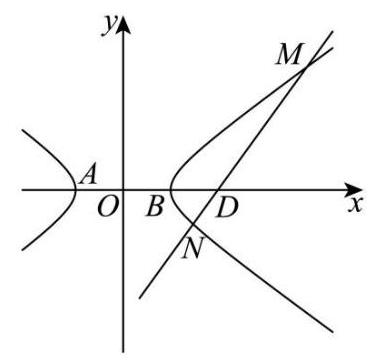
\includegraphics[max width=0.3\textwidth]{images/bo_d7ffgrqlb0pc73deo6k0_11_1145_1388_373_360_0.jpg}
\end{center}

\textbf{【答案】} \(\left( 1\right) \sqrt{5};\left( 2\right) \left( {2,3}\right)\) 或 \(\left( {\frac{5}{4},\frac{3\sqrt{3}}{4}}\right) ;\left( 3\right) \left( {\arctan \frac{\sqrt{2}}{2},\arctan \frac{\sqrt{10}}{2}}\right)\)

\textbf{【解析】}(1) 由题, \({2c} = 2\sqrt{5}\) ,得 \(c = \sqrt{5}\)

故 \(e = \frac{c}{a} = \sqrt{5}\)

(2)因为点 \(M\) 在第一象限，故 \(\angle {MAD}\) 不可能为直角；

若 \(\angle {ADM} = \frac{\pi }{2}\) ，将 \(x = 2\) 代入曲线 \(C : {x}^{2} - \frac{{y}^{2}}{3} = 1\) ，得 \(M\left( {2,3}\right)\) ；

若 \(\angle {DMA} = \frac{\pi }{2}\) ，设点 \(M\left( {{x}_{0},{y}_{0}}\right)\) ，则 \(\overrightarrow{MD} = \left( {2 - {x}_{0}, - {y}_{0}}\right) ,\overrightarrow{MA} = \left( {-1 - {x}_{0}, - {y}_{0}}\right)\) ，

则 \(\overrightarrow{MD} \cdot  \overrightarrow{MA} = {x}_{0}^{2} - {x}_{0} - 2 + {y}_{0}^{2} = 0\)

又因为点 \(M\) 满足 \({x}_{0}^{2} - \frac{{y}_{0}^{2}}{3} = 1\) ,可得 \(M\left( {\frac{5}{4},\frac{3\sqrt{3}}{4}}\right)\) .

综上,点 \(M\) 的坐标 \(\left( {2,3}\right)\) 或 \(\left( {\frac{5}{4},\frac{3\sqrt{3}}{4}}\right)\) ;

(3)由题可得，双曲线 \(C : {x}^{2} - 2{y}^{2} = 1\) ，

当直线 \(l\) 的斜率不存在时,根据双曲线的对称性, \(\overrightarrow{MN} = 2\overrightarrow{MD}\) ,不满足 \(\lambda  < \frac{4}{3}\) ,

所以直线 \(l\) 的斜率一定存在,

又 \(\overrightarrow{MN} = \lambda \overrightarrow{MD}\) ,说明 \(M, D, N\) 三点共线,且 \(M, N\) 都在双曲线的右支上,

所以直线 \(l\) 的斜率不为 \(0,1 < \lambda  < \frac{4}{3}\) ,

设直线 \(l\) 的方程为 \(x = {my} + 2, M\left( {{x}_{1},{y}_{1}}\right) \text{ 、 }N\left( {{x}_{2},{y}_{2}}\right)\) ,且 \({y}_{1} > 0,{y}_{2} < 0\) ,

联立方程 \(\left\{  \begin{array}{l} x = {my} + 2 \\  {x}^{2} - 2{y}^{2} = 1 \end{array}\right.\) ,可得 \(\left( {{m}^{2} - 2}\right) {y}^{2} + {4my} + 3 = 0\)

显然 \({m}^{2} - 2 \neq  0,\Delta  = {\left( 4m\right) }^{2} - 4\left( {{m}^{2} - 2}\right)  \times  3 = 4{m}^{2} + {24} > 0\) ,

\({y}_{1} + {y}_{2} = \frac{-{4m}}{{m}^{2} - 2} > 0,\;{y}_{1}{y}_{2} = \frac{3}{{m}^{2} - 2} < 0\) ,故 \(0 < m < \sqrt{2}\)

由 \(\overrightarrow{MN} = \lambda \overrightarrow{MD}\) ,可得 \({y}_{2} - {y}_{1} =  - \lambda {y}_{1}\) ,且 \(1 < \lambda  < \frac{4}{3}\) .

故 \(\frac{{y}_{2}}{{y}_{1}} = 1 - \lambda  \in  \left( {-\frac{1}{3},0}\right)\)

因此 \(\frac{{\left( {y}_{1} + {y}_{2}\right) }^{2}}{{y}_{1}{y}_{2}} = \frac{{y}_{2}}{{y}_{1}} + \frac{{y}_{1}}{{y}_{2}} + 2\) ,

根据对勾函数性质: 在 \(\left( {-1,0}\right)\) 上单调递减,

可知 \(\frac{{\left( {y}_{1} + {y}_{2}\right) }^{2}}{{y}_{1}{y}_{2}} <  - \frac{1}{3} + \left( {-3}\right)  + 2 =  - \frac{4}{3}\) ,

又 \(\frac{{\left( {y}_{1} + {y}_{2}\right) }^{2}}{{y}_{1}{y}_{2}} = {\left( -\frac{4m}{{m}^{2} - 2}\right) }^{2} \cdot  \frac{{m}^{2} - 2}{3} = \frac{16}{3} \cdot  \frac{{m}^{2}}{{m}^{2} - 2}\) ,

故 \(\frac{16}{3} \cdot  \frac{{m}^{2}}{{m}^{2} - 2} <  - \frac{4}{3}\) ,可得 \(\frac{2}{\sqrt{10}} < m < \sqrt{2}\) .

所以,直线 \(l\) 斜率的取值范围为 \(\left( {\frac{\sqrt{2}}{2},\frac{\sqrt{10}}{2}}\right)\) ,

直线 \(l\) 倾斜角的取值范围为 \(\left( {\arctan \frac{\sqrt{2}}{2},\arctan \frac{\sqrt{10}}{2}}\right)\) .

\begin{analysisbox}[考点分析]
\textbf{知识点}：双曲线、直线与圆锥曲线\\
\textbf{难度}：\(\star\star\star\star\) 压轴题\\
\textbf{评价}：圆锥曲线综合题，解答题压轴题之一。
\begin{itemize}
\item 第(1)问：基本量计算，由 \(2c = 2\sqrt{5}\) 求离心率
\item 第(2)问：分类讨论直角三角形的直角顶点位置
\item 第(3)问：向量关系转化为坐标关系，利用韦达定理
\item 关键：将对勾函数性质与不等式结合求范围
\end{itemize}
\end{analysisbox}

\begin{tipbox}[教学提示]
圆锥曲线大题的解题框架：
\begin{enumerate}
\item 第(1)(2)问通常是基础计算，确保得分
\item 第(3)问涉及范围问题时：
  \begin{itemize}
  \item 设直线方程（注意讨论斜率是否存在）
  \item 联立方程，利用韦达定理
  \item 将几何条件转化为代数不等式
  \item 利用函数性质（如对勾函数）求范围
  \end{itemize}
\item 向量条件的处理：转化为坐标之间的比例关系
\end{enumerate}
\end{tipbox}

\newpage

21. （19分）对于定义在区间 \(D\) 上的函数 \(y = f\left( x\right)\) ,定义集合 \(\Omega  = \left\{  {f\left( x\right) \begin{Vmatrix}{f\left( {x}_{1}\right)  - f\left( {x}_{2}\right) }\end{Vmatrix} \leq  \left| {{x}_{1} - {x}_{2}}\right| ,\forall {x}_{1},{x}_{2} \in  D}\right\}\) . 对任意闭区间 \(I \subseteq  D\) ,设函数 \(y = f\left( x\right)\) 在区间 \(I\) 上的最大值为 \({M}_{1}\) ,最小值为 \({M}_{2}\) ,记 \(M\left( {f,I}\right)  = {M}_{1} - {M}_{2}\) .

(1)若 \(f\left( x\right)  = {x}^{2} - x,D = \left\lbrack  {0,1}\right\rbrack\) ,判断函数 \(y = f\left( x\right)\) 是否属于集合 \(\Omega\) ,并求 \(M\left( {f,\left\lbrack  {0,1}\right\rbrack  }\right)\) 的值;

(2)若 \(D = \left\lbrack  {0,1}\right\rbrack  ,f\left( x\right)  \in  \Omega\) ,且 \(f\left( 0\right)  = 0,M\left( {f,\left\lbrack  {0,1}\right\rbrack  }\right)  = 1\) . 求 \(f\left( 1\right)\) 的值及函数 \(y = f\left( x\right)\) 的解析式;

(3)若 \(D = \lbrack 0, + \infty ),f\left( x\right)  \in  \Omega\) ,令 \(g\left( x\right)  = M\left( {f,\left\lbrack  {0,x}\right\rbrack  }\right)\) . 证明: \(y = f\left( x\right)\) 是单调函数的充要条件是: 对任意 \(0 < {x}_{1} < {x}_{2},\;g\left( {x}_{2}\right)  - g\left( {x}_{1}\right)  = M\left( {f,\left\lbrack  {{x}_{1},{x}_{2}}\right\rbrack  }\right)\) 恒成立.

\textbf{【答案】}(1)是, \(M\left( {f,\left\lbrack  {0,1}\right\rbrack  }\right)  = \frac{1}{4}\) ; (2)当 \(f\left( 1\right)  = 1\) 时, \(f\left( x\right)  = x\) ,当 \(f\left( 1\right)  =  - 1\) 时; \(f\left( x\right)  =  - x\) ; (3)见解析

\textbf{【解析】}(1) 对任意 \({x}_{1},{x}_{2} \in  \left\lbrack  {0,1}\right\rbrack\) ,所以 \(0 \leq  {x}_{1} + {x}_{2} \leq  2, - 1 \leq  {x}_{1} + {x}_{2} - 1 \leq  1\) , 又因为 \(\left| {f\left( {x}_{1}\right)  - f\left( {x}_{2}\right) }\right|  = \left| {\left( {{x}_{1}^{2} - {x}_{1}}\right)  - \left( {{x}_{2}^{2} - {x}_{2}}\right) }\right|  = \left| {\left( {{x}_{1}^{2} - {x}_{2}^{2}}\right)  - \left( {{x}_{1} - {x}_{2}}\right) }\right|  = \left| {{x}_{1} - {x}_{2}}\right|  \cdot  \left| {{x}_{1} + {x}_{2} - 1}\right|\) ,且 \({x}_{1} + {x}_{2} - 1 \in  \left\lbrack  {-1,1}\right\rbrack\) , 所以 \(\left| {f\left( {x}_{1}\right)  - f\left( {x}_{2}\right) }\right|  \leq  \left| {{x}_{1} - {x}_{2}}\right|\) ,故函数 \(y = f\left( x\right)\) 属于集合 \(\Omega\) .

由 \(f\left( x\right)  = {x}^{2} - x = {\left( x - \frac{1}{2}\right) }^{2} - \frac{1}{4}, x \in  \left\lbrack  {0,1}\right\rbrack\) ,由二次函数的性质可知 \({M}_{1} = f\left( 0\right)  = f\left( 1\right)  = 0,{M}_{2} = f\left( \frac{1}{2}\right)  =  - \frac{1}{4}\) . 故 \(M\left( {f,\left\lbrack  {0,1}\right\rbrack  }\right)  = \frac{1}{4}\) .

(2)由 \(M\left( {f,\left\lbrack  {0,1}\right\rbrack  }\right)  = 1\) 可知，存在 \(u, v \in  \left\lbrack  {0,1}\right\rbrack\) 满足 \(\left| {f\left( u\right)  - f\left( v\right) }\right|  = 1\) .

又 \(f\left( x\right)  \in  \Omega\) ,故必有 \(\left| {f\left( u\right)  - f\left( v\right) }\right|  \leq  \left| {u - v}\right|  \leq  1\) .

因此必有 \(\left| {u - v}\right|  = 1\) ,且 \(u, v \in  \left\lbrack  {0,1}\right\rbrack\) ,所以 \(\{ u, v\}  = \{ 0,1\}\) ,

又 \(f\left( 0\right)  = 0,\left| {f\left( 1\right)  - f\left( 0\right) }\right|  = 1\) ,所以 \(f\left( 1\right)  = 1\) 或 \(f\left( 1\right)  =  - 1\)

当 \(f\left( 1\right)  = 1\) 时,由题意,对任意 \(x \in  \left\lbrack  {0,1}\right\rbrack  ,\left| {f\left( x\right)  - f\left( 0\right) }\right|  \leq  x,\left| {f\left( x\right) }\right|  \leq  x\) ,即 \(f\left( x\right)  \leq  x\) .

又因为 \(\left| {f\left( 1\right)  - f\left( x\right) }\right|  \leq  1 - x\) ,即 \(1 - f\left( x\right)  \leq  1 - x\) ,故 \(f\left( \mathrm{x}\right)  \geq  \mathrm{x}\) .

故 \(f\left( x\right)  = x\) .

当 \(f\left( 1\right)  =  - 1\) 时,由题意,对任意 \(x \in  \left\lbrack  {0,1}\right\rbrack  ,\left| {f\left( x\right)  - f\left( 0\right) }\right|  \leq  x,\left| {f\left( x\right) }\right|  \leq  x\) ,即 \(f\left( x\right)  \geq   - x\) ,

又因为 \(\left| {f\left( x\right)  - f\left( 1\right) }\right|  \leq  1 - x,\left| {f\left( x\right)  + 1}\right|  \leq  1 - x\) ,即 \(f\left( x\right)  + 1 \leq  1 - x\) ,故 \(f\left( x\right)  \leq   - x\)

所以 \(f\left( x\right)  =  - x.\)

综上,当 \(f\left( 1\right)  = 1\) 时, \(f\left( x\right)  = x\) ; 当 \(f\left( 1\right)  =  - 1\) 时; \(f\left( x\right)  =  - x\) .

(3)先证必要性:若 \(y = f\left( x\right)\) 是定义在 \(\lbrack 0, + \infty )\) 上的增函数，

设任意正实数 \({X}_{1}\text{ 、 }{X}_{2}\) 满足 \(0 < {x}_{1} < {x}_{2}\) ,

则 \(g\left( {x}_{2}\right)  = M\left( {f,\left\lbrack  {0,{x}_{2}}\right\rbrack  }\right)  = f\left( {x}_{2}\right)  - f\left( 0\right) , g\left( {x}_{1}\right)  = f\left( {x}_{1}\right)  - f\left( 0\right) , M\left( {f,\left\lbrack  {{x}_{1},{x}_{2}}\right\rbrack  }\right)  = f\left( {x}_{2}\right)  - f\left( {x}_{1}\right)\) .

因此 \(g\left( {x}_{2}\right)  - g\left( {x}_{1}\right)  = f\left( {x}_{2}\right)  - f\left( {x}_{1}\right)  = M\left( {f,\left\lbrack  {{x}_{1},{x}_{2}}\right\rbrack  }\right)\) ,得证.

若 \(y = f\left( x\right)\) 是定义在 \(\lbrack 0, + \infty )\) 上的减函数,

设任意正实数 \({X}_{1}\text{ 、 }{X}_{2}\) 满足 \(0 < {x}_{1} < {x}_{2}\) ,

则 \(g\left( {x}_{2}\right)  = M\left( {f,\left\lbrack  {0,{x}_{2}}\right\rbrack  }\right)  = f\left( 0\right)  - f\left( {x}_{2}\right) , g\left( {x}_{1}\right)  = f\left( 0\right)  - f\left( {x}_{1}\right) , M\left( {f,\left\lbrack  {{x}_{1},{x}_{2}}\right\rbrack  }\right)  = f\left( {x}_{1}\right)  - f\left( {x}_{2}\right)\) .

因此 \(g\left( {x}_{2}\right)  - g\left( {x}_{1}\right)  = \left\lbrack  {f\left( 0\right)  - f\left( {x}_{2}\right) }\right\rbrack   - \left\lbrack  {f\left( 0\right)  - f\left( {x}_{1}\right) }\right\rbrack   = f\left( {x}_{1}\right)  - f\left( {x}_{2}\right)  = M\left( {f,\left\lbrack  {{x}_{1},{x}_{2}}\right\rbrack  }\right)\) ,得证.

综上, 必要性得证.

再证充分性: (反证法) 假设函数 \(y = f\left( x\right)\) 在 \(\lbrack 0, + \infty )\) 上不单调,

则必存在 \({x}_{1} < {x}_{0} < {x}_{2}\) ,使得 \(f\left( {x}_{1}\right) < f\left( {x}_{0}\right) > f\left( {x}_{2}\right)\) 或 \(f\left( {x}_{1}\right)  > f\left( {x}_{0}\right)  < f\left( {x}_{2}\right)\) .

不妨设 \(f\left( {x}_{1}\right) < f\left( {x}_{0}\right) > f\left( {x}_{2}\right)\) ,且 \(f\left( {x}_{0}\right)\) 是函数 \(y = f\left( x\right)\) 在区间 \(\left\lbrack  {{x}_{1},{x}_{2}}\right\rbrack\) 上的最大值.

设函数 \(y = f\left( x\right)\) 在区间 \(\left\lbrack  {{x}_{1},{x}_{0}}\right\rbrack\) 上的最小值为 \({L}_{1}\) ,在区间 \(\left\lbrack  {{x}_{0},{x}_{2}}\right\rbrack\) 上的最小值为 \({L}_{2}\)

由题, \(M\left( {f,\left\lbrack  {{x}_{1},{x}_{0}}\right\rbrack  }\right)  = g\left( {x}_{0}\right)  - g\left( {x}_{1}\right) , M\left( {f,\left\lbrack  {{x}_{0},{x}_{2}}\right\rbrack  }\right)  = g\left( {x}_{2}\right)  - g\left( {x}_{0}\right)\) ,

故 \(M\left( {f,\left\lbrack  {{x}_{1},{x}_{0}}\right\rbrack  }\right)  + M\left( {f,\left\lbrack  {{x}_{0},{x}_{2}}\right\rbrack  }\right)  = g\left( {x}_{2}\right)  - g\left( {x}_{1}\right)\) ,又 \(g\left( {x}_{2}\right)  - g\left( {x}_{1}\right)  = M\left( {f,\left\lbrack  {{x}_{1},{x}_{2}}\right\rbrack  }\right)\) ,

故 \(M\left( {f,\left\lbrack  {{x}_{1},{x}_{0}}\right\rbrack  }\right)  + M\left( {f,\left\lbrack  {{x}_{0},{x}_{2}}\right\rbrack  }\right)  = M\left( {f,\left\lbrack  {{x}_{1},{x}_{2}}\right\rbrack  }\right)\)

即 \(f\left( {x}_{0}\right)  - {L}_{1} + f\left( {x}_{0}\right)  - {L}_{2} = f\left( {x}_{0}\right)  - \min \left\{  {{L}_{1},{L}_{2}}\right\}\) ,

即 \(f\left( {x}_{0}\right)  = {L}_{1} + {L}_{2} - \min \left\{  {{L}_{1},{L}_{2}}\right\}\) ,即 \(f\left( {x}_{0}\right)  = \max \left\{  {{L}_{1},{L}_{2}}\right\}\) ,

\(\max \left\{  {{L}_{1},{L}_{2}}\right\}   \leq  \max \left\{  {f\left( {x}_{1}\right) , f\left( {x}_{2}\right) }\right\}   < f\left( {x}_{0}\right)\) ,矛盾.

因此假设不成立. \(f\left( x\right)\) 是 \(\lbrack 0, + \infty )\) 上的单调函数.

因此, \(y = f\left( x\right)\) 是单调函数的充要条件是: 对任意正实数 \(0 < {x}_{1} < {x}_{2}\) ,

\(g\left( {x}_{2}\right)  - g\left( {x}_{1}\right)  = M\left( {f,\left\lbrack  {{x}_{1},{x}_{2}}\right\rbrack  }\right)\) 恒成立。

\begin{analysisbox}[考点分析]
\textbf{知识点}：函数性质、充要条件证明\\
\textbf{难度}：\(\star\star\star\star\) 压轴题\\
\textbf{评价}：新定义函数题，试卷压轴题。
\begin{itemize}
\item 第(1)问：验证Lipschitz条件，求函数在区间上的最大值差
\item 第(2)问：利用夹逼思想确定函数解析式，只能是 \(f(x) = x\) 或 \(f(x) = -x\)
\item 第(3)问：充要条件证明，必要性直接验证，充分性用反证法
\item 核心：理解 \(M(f, I)\) 的几何意义——函数在区间上的"振幅"
\end{itemize}
\end{analysisbox}

\begin{tipbox}[教学提示]
新定义压轴题的应对策略：
\begin{enumerate}
\item 耐心阅读定义，用自己的话复述一遍
\item 从简单情形入手（如第1问的二次函数）建立直觉
\item 第(2)问的夹逼思想：\(|f(x)| \leq x\) 且 \(|f(x) - f(1)| \leq 1-x\) 联立
\item 充要条件证明的标准格式：分必要性和充分性两部分
\item 反证法的关键：找到矛盾点（本题是最大值的位置矛盾）
\end{enumerate}
\end{tipbox}

\vfill
\begin{center}
\rule{0.5\textwidth}{0.4pt}\\[0.5em]
\textit{— 试卷解析结束 —}\\[0.3em]
\small 本解析版包含详细考点分析与教学评价，供教师备课参考
\end{center}

\end{document}
